\documentclass[11pt,a4paper]{article}
\usepackage[utf8]{inputenc}
\usepackage[margin=1in]{geometry}
\usepackage{amsmath,amssymb}
\usepackage{hyperref}
\usepackage{graphicx}
\usepackage{booktabs}
\usepackage{enumitem}
\usepackage{tikz}
\usetikzlibrary{shapes.geometric, arrows.meta, positioning}

% Hyperlink Setup
\hypersetup{
    colorlinks=true,
    linkcolor=blue,
    citecolor=blue,
    urlcolor=blue
}

\title{\textbf{Project Proposal (v2)}\\[0.5em] 
\Large Multi-Scale Integration of Macroscopic fMRI and Mesoscopic Attractor Circuit Models: Decoding Working Memory Modulation of Visual and Auditory Representations}
\author{}
\date{\today}

\begin{document}

\maketitle

\hrule
\vspace{1em}

\section{Motivation \& Background}

A central challenge in cognitive neuroscience is bridging the gap between macroscopic neuroimaging observations and mesoscopic computational mechanisms. While task-based functional Magnetic Resonance Imaging (fMRI) excels at mapping cognitive functions to specific brain networks, the Blood Oxygen Level Dependent (BOLD) signal reflects metabolic energy consumption averaged over millions of neurons and several seconds. Consequently, standard univariate fMRI cannot explain \textit{how} information is dynamically encoded, maintained, and manipulated at the microcircuit level.

In working memory (WM), the classical paradigm assumes that information is maintained through persistent, high-frequency spiking in frontal-parietal circuits. However, persistent spiking is metabolically expensive and susceptible to distraction. Recent biophysical theories, specifically \textbf{Short-Term Synaptic Plasticity (STSP)} based on Tsodyks-Markram dynamics, propose an alternative ``activity-silent'' mechanism. Under STSP, memory items are encoded in transient changes in presynaptic calcium utilization ($u$) and available neurotransmitter resources ($x$), allowing representations to be maintained with minimal spiking during delay intervals.

A further open question is whether these mechanisms are specific to the sensory modality of the stimulus. Visual category information is carried by occipito-temporal cortex, whereas auditory (speech and language) information is carried by Heschl's gyrus and the superior temporal cortex. In contrast, the multiple-demand view of frontoparietal cortex holds that executive control regions are recruited across sensory modalities. Testing visual and auditory data side by side therefore allows a direct comparison between \textbf{modality-specific sensory representations} and \textbf{modality-general control signals}, and provides a stronger constraint on the circuit model than visual data alone.

This project addresses this methodological scale gap by establishing a quantitative, closed-loop pipeline. By integrating \textbf{Human Connectome Project (HCP)} task fMRI from the visual working memory task (\texttt{tfMRI\_WM}) and the auditory language task (\texttt{tfMRI\_LANGUAGE}) with \textbf{Representational Similarity Analysis (RSA)}, \textbf{Multivariate Pattern Analysis (MVPA)}, and \textbf{Leaky Integrate-and-Fire (LIF)} attractor network modeling, this project directly connects localized BOLD metabolic demands to specific information content and synaptic calcium dynamics in both modalities.

\section{Detailed Problem Statement}

Univariate General Linear Model (GLM) analyses consistently demonstrate that high working memory load (e.g., 2-back vs. 0-back) increases BOLD activation across the Frontoparietal/Cingulate control network and modulates activity in visual cortices. Auditory tasks with higher cognitive demand (e.g., arithmetic vs. story comprehension in the HCP language task) are likewise reported to recruit frontoparietal regions in addition to auditory cortex. However, univariate methods suffer from key theoretical limitations:

\begin{enumerate}
    \item \textbf{Univariate Ambiguity:} Increased BOLD activation in frontoparietal regions could reflect top-down gain control, non-specific attentional recruitment, or the active maintenance of category-specific contents.
    \item \textbf{Representational Geometry under Load:} It remains unresolved whether cognitive load distorts the underlying representational geometry (pairwise dissimilarity) of visual category targets in visual cortices or leaves it structurally invariant.
    \item \textbf{Metabolic-Circuit Gap:} There is no standard framework to prove whether empirical fMRI BOLD parameter estimates ($\beta$) in executive regions match the theoretical metabolic costs of activity-silent STSP maintenance (periodic population refreshes and calcium pump clearance).
    \item \textbf{Modality Specificity vs. Generality:} Univariate contrasts cannot determine whether the demand-related signal in frontoparietal cortex is shared across visual and auditory input, or whether it is a separate code for each modality.
\end{enumerate}

\subsection*{Core Research Hypotheses}

\begin{itemize}
    \item \textbf{Hypothesis 1 ($H_1$):} Visual category representations in Occipito-Temporal cortex maintain structural geometric invariance across working memory load states (0-back vs. 2-back).
    \item \textbf{Hypothesis 2 ($H_2$):} Category-specific information emerges dynamically in Frontoparietal/Cingulate control regions under high working memory load (2-back), even if these regions show no category tuning during passive viewing (0-back).
    \item \textbf{Hypothesis 3 ($H_3$):} The theoretical metabolic expenditure (ATP) of periodic population bursts and presynaptic calcium clearance in a simulated STSP circuit quantitatively accounts for the empirical BOLD $\beta$ magnitude observed in task fMRI, for both the visual and the auditory condition.
    \item \textbf{Hypothesis 4 ($H_4$):} Sensory cortices are modality-specific, whereas control regions are modality-general: a high- versus low-demand pattern learned in the visual task (2-back vs. 0-back) transfers to the auditory task (Math vs. Story) in Frontoparietal/Cingulate cortex, but not in Occipito-Temporal or Auditory cortex.
\end{itemize}

\section{Methodology, Simulation Protocol, \& Expected Results}

The project is structured into a sequential three-phase workflow pipeline:

\begin{center}
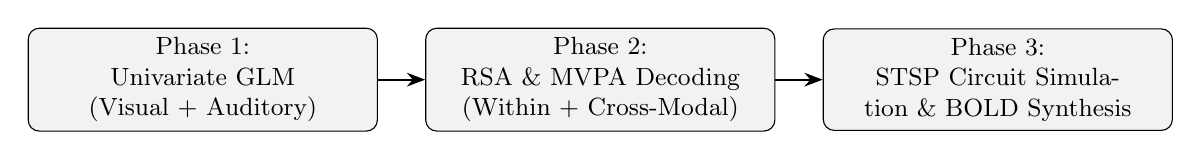
\begin{tikzpicture}[
    node distance=0.6cm, 
    auto, 
    >=Stealth,
    phase/.style={draw, rectangle, rounded corners, align=center, fill=gray!10, text width=4.2cm, font=\small, minimum height=1cm}
]
    \node [phase] (phase1) {Phase 1:\\Univariate GLM\\(Visual + Auditory)};
    \node [phase, right=of phase1] (phase2) {Phase 2:\\RSA \& MVPA Decoding\\(Within + Cross-Modal)};
    \node [phase, right=of phase2] (phase3) {Phase 3:\\STSP Circuit Simulation \& BOLD Synthesis};
    
    \draw [->, thick] (phase1) -- (phase2);
    \draw [->, thick] (phase2) -- (phase3);
\end{tikzpicture}
\end{center}

\subsection{Phase 1: Signal Extraction \& First-Level GLM Fitting}

\begin{itemize}
    \item \textbf{Data Processing:} Process Left-Right (LR) and Right-Left (RL) phase encoding runs from two HCP task datasets: the visual \texttt{tfMRI\_WM} working memory task and the auditory \texttt{tfMRI\_LANGUAGE} task (TR $\approx$ 0.7s, 2mm isotropic MNI space). In the language task, stimuli (short stories and arithmetic problems) are presented through headphones, which makes it the auditory counterpart of the visual WM task. The same subject subset is used for both tasks.
    \item \textbf{Nuisance \& EV Modeling:} Parse 8 visual experimental Explanatory Variable (EV) conditions:
    \[
    \text{Load } (0\text{-back}, 2\text{-back}) \times \text{Category } (\text{Body}, \text{Face}, \text{Place}, \text{Tool})
    \]
    and 2 auditory block conditions from the language task (Story, Math), giving 10 conditions in total. Extract 6 rigid-body motion parameters (translation and rotation) as nuisance regressors for every run.
    \item \textbf{GLM Contrast Extraction:} Fit a Nilearn \texttt{FirstLevelModel} using a Glover HRF and AR(1) noise model separately for each task, to generate 8 raw effect-size ($\beta$) maps per run for the visual task and 2 per run for the auditory task, all relative to implicit fixation/baseline.
    \item \textbf{ROI Definition:} Define binary masks for Occipito-Temporal (category-selective visual), Auditory (Heschl's gyrus, planum temporale and superior temporal gyrus) and Frontoparietal/Cingulate (load-sensitive control) regions using the Harvard-Oxford probabilistic atlas resampled to the subject BOLD geometry.
\end{itemize}

\subsection{Phase 2: Information Representation (RSA \& Decoding)}

\begin{itemize}
    \item \textbf{Split-Half RSA (Step 4):} Compute cross-run ($LR \leftrightarrow RL$) Pearson dissimilarity matrices ($D = 1 - r$) across the 10 conditions to generate $10 \times 10$ RDMs (visual block $8 \times 8$, auditory block $2 \times 2$, plus the visual--auditory cross-block). Extract $4 \times 4$ category sub-RDMs for 0-back and 2-back conditions. Compare the visual and auditory blocks within each ROI to quantify how strongly each region separates the two modalities.
    \item \textbf{Targeted Gap Test ($H_1$):} Calculate the Spearman rank correlation ($\rho$) between the upper-triangular off-diagonal vectors of the 0-back and 2-back category sub-RDMs to evaluate representational invariance under load.
    \item \textbf{Linear MVPA Decoding (Step 5):} Train Linear Support Vector Machines (SVM) with cross-run fold validation ($LR \leftrightarrow RL$) to perform:
    \begin{enumerate}
        \item 4-way Category Decoding within 0-back and 2-back (Chance = 25\%).
        \item 2-way Binary Load Decoding (0-back vs. 2-back, Chance = 50\%).
        \item Cross-Load Category Generalization (Train on 0-back $\rightarrow$ Test on 2-back) to test $H_2$.
        \item 2-way Auditory Decoding (Story vs. Math, Chance = 50\%) in Auditory and Frontoparietal/Cingulate ROIs.
        \item 2-way Modality Decoding (visual vs. auditory blocks, Chance = 50\%) in each ROI, as a sanity check that sensory ROIs are modality-specific.
        \item Cross-Modal Demand Generalization (Train on visual 2-back vs. 0-back $\rightarrow$ Test on auditory Math vs. Story, and the reverse) to test $H_4$.
    \end{enumerate}
\end{itemize}

\subsection{Phase 3: Biophysical STSP Circuit Simulation \& BOLD Synthesis}

\begin{itemize}
    \item \textbf{Network Initialization (Step 6):} Construct a biophysical spiking network representing a frontoparietal cortical column containing $N_E = 800$ excitatory pyramidal neurons and $N_I = 200$ inhibitory interneurons. Partition $N_E$ into 4 visual category-selective pools, 2 auditory pools (Story, Math) (100 units/pool) and 1 background pool (200 units). Scale intra-pool recurrent gain ($w_+$) using empirical decoding performance from Step 5, separately for the visual and auditory pools.
    \item \textbf{Synaptic Dynamics Simulation (Step 7):} Simulate Leaky Integrate-and-Fire (LIF) membrane dynamics alongside Tsodyks-Markram STSP differential equations:
    \begin{align}
        \frac{du}{dt} &= \frac{U_{\text{baseline}} - u}{\tau_F} + U_{\text{baseline}}(1 - u) \sum_k \delta(t - t_k) \\
        \frac{dx}{dt} &= \frac{1 - x}{\tau_D} - u \cdot x \sum_k \delta(t - t_k)
    \end{align}
    Simulate the 2-back maintenance delay (cue presentation $\rightarrow$ activity-silent delay) driven through a visual pool, and the corresponding high-demand (Math) and low-demand (Story) auditory epochs driven through an auditory pool, to model $u$ (calcium utilization) and $x$ (resource availability) in each case.
    \item \textbf{LFP \& BOLD Synthesis (Step 8):}
    \begin{enumerate}
        \item Compute Local Field Potentials (LFPs) as aggregate synaptic fluxes and extract Theta (4--8 Hz) and Gamma (30--80 Hz) power spectra using continuous spectrograms.
        \item Calculate total metabolic ATP expenditure ($ATP_{\text{total}}$) combining action potential costs ($C_{\text{AP}}$) and calcium pump clearance costs ($C_{\text{Ca}}$):
        \[
        ATP_{\text{total}}(t) = N_{\text{spikes}}(t) \cdot C_{\text{AP}} + \sum_{i \in E} \max\left(0, \frac{du_i}{dt}\right) \cdot C_{\text{Ca}}
        \]
        \item Convolve $ATP_{\text{total}}(t)$ with a double-gamma Glover HRF to synthesize the predicted BOLD time-series and compare its peak magnitude directly against the empirical First-Level GLM $\beta$ estimate, for the visual and the auditory condition.
    \end{enumerate}
\end{itemize}

\begin{center}
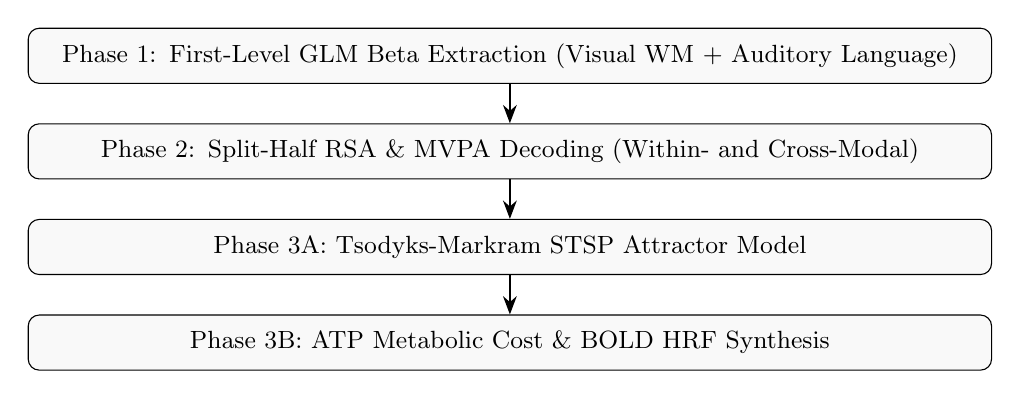
\begin{tikzpicture}[
    node distance=0.5cm, 
    auto, 
    >=Stealth, 
    block/.style={draw, rectangle, rounded corners, align=center, fill=gray!5, text width=12cm, font=\small, minimum height=0.7cm}
]
    \node [block] (step1) {Phase 1: First-Level GLM Beta Extraction (Visual WM + Auditory Language)};
    \node [block, below=of step1] (step2) {Phase 2: Split-Half RSA \& MVPA Decoding (Within- and Cross-Modal)};
    \node [block, below=of step2] (step3) {Phase 3A: Tsodyks-Markram STSP Attractor Model};
    \node [block, below=of step3] (step4) {Phase 3B: ATP Metabolic Cost \& BOLD HRF Synthesis};
    
    \draw [->, thick] (step1) -- (step2);
    \draw [->, thick] (step2) -- (step3);
    \draw [->, thick] (step3) -- (step4);
\end{tikzpicture}
\end{center}

\subsection{Expected Results}

\begin{enumerate}
    \item \textbf{Occipito-Temporal Structural Invariance:} High Spearman rank correlation ($\rho > 0.85, p < 0.001$) between 0-back and 2-back category sub-RDMs in visual cortices, confirming representational invariance under cognitive load ($H_1$).
    \item \textbf{Frontoparietal Dynamic Emergence:} Category decoding accuracy in Frontoparietal cortex rises significantly above chance (25\%) strictly during the 2-back condition, confirming load-dependent recruitment of executive regions for content maintenance ($H_2$).
    \item \textbf{Activity-Silent Memory Trajectory:} Following cue offset, spiking activity in the simulated circuit returns to baseline while synaptic efficacy ($u \cdot x$) remains elevated for $>1500\text{ ms}$, demonstrating silent chemical storage.
    \item \textbf{Model-Data BOLD Alignment:} Synthesized BOLD signals derived from simulated ATP expenditure (spikes + calcium clearance) match empirical GLM $\beta$ magnitudes within a tight ratio ($0.90 - 1.10$) for both the visual and auditory conditions, validating the biophysical origin of the fMRI signal ($H_3$).
    \item \textbf{Modality-Specific Sensory Codes:} Visual-vs-auditory decoding is near ceiling in Occipito-Temporal and Auditory cortex, and Story-vs-Math decoding in Auditory cortex is significantly above chance (50\%), confirming the sensory ROIs carry modality-specific information.
    \item \textbf{Modality-General Control Signal:} Cross-modal demand generalization (visual $\rightarrow$ auditory and the reverse) is significantly above chance (50\%, permutation test) in Frontoparietal/Cingulate cortex but at chance in sensory ROIs ($H_4$).
\end{enumerate}

\section{Novelty, Key References, Code \& Data Repositories}

\subsection{Project Novelty}

\begin{enumerate}
    \item \textbf{Closed-Loop Multi-Scale Bridge:} Unlike standard neuroimaging studies that stop at MVPA decoding, or computational studies that rely on arbitrary network parameters, this project establishes a direct quantitative loop: empirical MVPA performance constrains recurrent attractor gain ($w_+$), and simulated biophysical ATP costs predict empirical fMRI $\beta$ weights.
    \item \textbf{Activity-Silent BOLD Validation:} Provides an explicit metabolic account showing that activity-silent memory traces---maintained via calcium utilization ($u$) and brief refreshing bursts---generate measurable BOLD signals through presynaptic $\text{Ca}^{2+}$ clearance dynamics.
    \item \textbf{Cross-Load Generalization Analysis:} Formally tests the transferability of visual representational codes into executive control networks across differing working memory demands, as well as similarly testing the transferability of auditory representational codes across differing cognitive demands.
    \item \textbf{Cross-Modal (Visual--Auditory) Generalization:} Extends the analysis to auditory data and tests whether the executive demand code is shared across sensory modalities while sensory cortices stay modality-specific, using the same circuit model to account for the BOLD signal in both modalities.
\end{enumerate}

\subsection{Key References}

\begin{enumerate}[label={[\arabic*]}]
    \item Tsodyks, M. V., \& Markram, H. (1997). The neural code between neocortical pyramidal neurons depends on neurotransmitter release probability. \textit{Proceedings of the National Academy of Sciences}, 94(2), 719--723.
    \item Mongillo, G., Barak, O., \& Tsodyks, M. (2008). Synaptic theory of working memory. \textit{Science}, 319(5869), 1543--1546.
    \item Stokes, M. G. (2015). ‘Activity-silent’ working memory in prefrontal cortex: a dynamic coding framework. \textit{Trends in Cognitive Sciences}, 19(7), 394--405.
    \item Kriegeskorte, N., Mur, M., \& Bandettini, P. A. (2008). Representational similarity analysis–connecting the branches of systems neuroscience. \textit{Frontiers in Systems Neuroscience}, 2, 4.
    \item Barch, D. M., et al. (2013). Function in the human connectome: Task-fMRI and individual differences in behavior. \textit{NeuroImage}, 80, 169--189.
    \item Haxby, J. V., et al. (2001). Distributed and overlapping representations of faces and objects in ventral temporal cortex. \textit{Science}, 293(5539), 2425--2430.
    \item Binder, J. R., et al. (2011). Mapping anterior temporal lobe language areas with fMRI: A multicenter normative study. \textit{NeuroImage}, 54(2), 1465--1475.
    \item Duncan, J. (2010). The multiple-demand (MD) system of the primate brain: mental programs for intelligent behaviour. \textit{Trends in Cognitive Sciences}, 14(4), 172--179.
    \item Fedorenko, E., Duncan, J., \& Kanwisher, N. (2013). Broad domain generality in focal regions of frontal and parietal cortex. \textit{Proceedings of the National Academy of Sciences}, 110(41), 16616--16621.
\end{enumerate}

\subsection{Code \& Data Repositories}

\begin{itemize}
    \item \textbf{Primary Dataset:} Human Connectome Project (HCP) Young Adult 1200 Subjects Release (\texttt{tfMRI\_WM} Working Memory Task Dataset and \texttt{tfMRI\_LANGUAGE} auditory Story/Math Task Dataset, volume-space preprocessed NIfTI files and 3-column EV text files).
    \item \textbf{Software Stack \& Libraries:}
    \begin{itemize}
        \item \texttt{Python 3.8+}
        \item \texttt{Nilearn} (First-Level GLM modeling, atlas management, NiftiMasker pattern extraction)
        \item \texttt{NiBabel} (Neuroimaging NIfTI image manipulation)
        \item \texttt{Scikit-Learn} (Linear Support Vector Machines, StandardScaler, cross-validation pipelines)
        \item \texttt{SciPy} (Spearman rank correlation, spectrogram signal analysis, gamma distribution functions)
        \item \texttt{Pandas} / \texttt{NumPy} (EV table parsing, vector operations, Euler integration)
        \item \texttt{Matplotlib} / \texttt{Seaborn} (RDM heatmaps, raster plots, spectral and BOLD time-series visualization)
    \end{itemize}
    \item \textbf{Pipeline Code Repository Structure:}
    \begin{itemize}
        \item \texttt{Phase1\_GLM\_Condition\_Mapping.py}: EV parsing (visual WM and auditory language tasks), motion regression, and Nilearn FirstLevelModel fitting.
        \item \texttt{Phase1\_ROI\_Pattern\_Extraction.py}: Harvard-Oxford atlas masking (Occipito-Temporal, Auditory, Frontoparietal/Cingulate) and voxel pattern vector extraction.
        \item \texttt{Phase2\_Split\_Half\_RSA.py}: $10 \times 10$ cross-run RDM construction (visual, auditory and cross-modal blocks) and rank correlation testing.
        \item \texttt{Phase2\_MVPA\_Decoding.py}: 4-way category, 2-way load, Story-vs-Math, modality, and cross-load/cross-modal linear SVM decoding.
        \item \texttt{Phase3\_STSP\_Network\_Init.py}: Biophysical neuron pool setup (visual and auditory pools) and connectivity matrix ($W$) initialization.
        \item \texttt{Phase3\_STSP\_Synaptic\_Simulation.py}: LIF Euler integration and Tsodyks-Markram $u, x$ differential equation solver.
        \item \texttt{Phase3\_Synthesis\_BOLD\_Prediction.py}: LFP spectrogram generation, ATP metabolic cost calculation, and Glover HRF BOLD synthesis.
    \end{itemize}
\end{itemize}

\end{document}